\chapter{Subsystem Services}


\textbf{Controller Subsystem}\\\\
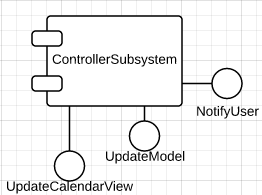
\includegraphics[scale=0.8]{ControllerServices}\\\\

The ControllerSubsystem is a subsystem that contains 3 different controllers:

\begin{itemize}
  \item ViewController
  \item InputController
  \item NotificationController
\end{itemize}

The purpose of our viewController is to change the view, depending on the interaction between the user and the system. There are different kinds of views, such as a view for login, event creation, the calendar as a whole and so on. Our UpdateCalendarView service will use the viewController to update the calendar view whenever there has been made a change in the calendar, for example if there has been added an event to the calendar.\\

The purpose of our InputController is to use the input that the system gets and then do something with the input, depending on the current event. The UpdateModel service will use the InputController to update the model, and thereby change the state of the model, and thereafter the UpdateCalendarView service will be used to update the calendar view with the new state of the model.\\

The purpose of our NotificationController is to notify the user, of a specific notification that has been set by the user. The NotifyUser service will be using the NotificationController to notify the user, which then will create a NotificationView that will be showed by the viewController to the user.\\


\textbf{Model Subsystem}\\\\
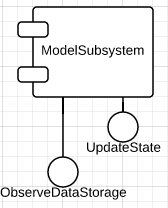
\includegraphics[scale=0.8]{ModelServices}\\\\

The ModelSubsystem consists of two different services: UpdateState and ObserveDataStorage.\\

Our UpdateState service is meant to update the state of the model, that the current system is using. When the UpdateModel service is being used by the ControllerSubsystem, the ModelSubsystem will receive whatever data that the UpdateModel service has to give, and then update its own state with the new data, received by the ControllerSubsystem, by using the UpdateState service.\\

Our ObserveDataStorage service is meant to observe and receive data from our persistent data storage, which is our database. When the user starts up our system, our ModelSubsystem will be using the ObserveDataStorage service to check if there is any updated data, that the current system doesn't contain, and if there are any updated data, it will receive that data from the database, store it locally and show it by using the ViewController.\\


\textbf{View Subsystem}\\\\
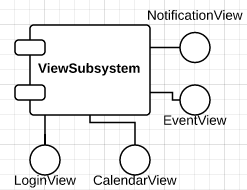
\includegraphics[scale=0.8]{ViewServices}\\\\

The ViewSubsystem contains four different services: NotificationView, EventView, CalendarView and LoginView.\\

As the ViewSubsystem services in themselves are views, the Subsystem services' purpose will be to create the different views, depending on the current event.\\


\textbf{DataStorage Subsystem}\\\\
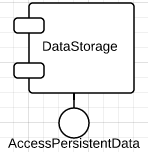
\includegraphics[scale=0.8]{DatastorageServices}\\\\

The DataStorage Subsystem contains a single service, which will be used to access the persistent data, that has been put into our database. This service will be used by our ObserveDataStorage service of our ModelSubsystem, to observe and receive data from the database, though our DataStorage Subsystem.